 \section{Results and Discussion}
In this section we present some of the results of our experiments and discuss their implications. We focus on the comparison between full-batch gradient descent (FGD) and stochastic gradient descent (SGD) in terms of convergence behavior and computational efficiency. Also we analyze the effects of different hyperparameters, such as the learning rate, the mini-batch size and the $L^2$ regularization parameter on the performance of SGD.

For evaluation, we use three disjoint subsets with the default proportions
\[
\text{train}=0.70,\qquad \text{val}=0.15,\qquad \text{test}=0.15.
\]
The split is computed with \emph{sklearn.model\_selection.train\_test\_split} using the \emph{stratify} option, so that each subset preserves (approximately) the original class proportions.


\subsection{Hyperparameter tuning}\;\\
In order to find good hyperparameters for our models, we followed the approach to tune them sequentially on the validation set. We are aware that this approach is not optimal, since the hyperparameters are not independent of each other and therefore it would be better to tune them jointly, e.g. by doing a grid search over the hyperparameter space. However we decided to follow this approach for simplicity.

\subsubsection{$L^2$ regularization}\;\\
To select the $L^2$ regularization strength, we ran SGD with fixed $\alpha=0.5$ and $B=64$ over a grid of $\lambda$ values and compared the resulting validation accuracy (Figure~\ref{fig:learning_rate_tuning}). The effect of regularization is clearly visible: accuracy remains essentially unchanged for very small $\lambda$, while it deteriorates as $\lambda$ becomes larger (around $10^{-4}$--$10^{-2}$). This behavior is consistent with the bias--variance trade-off: moderate regularization can help control overfitting, but overly large $\lambda$ penalizes the weights too strongly, leading to underfitting and reduced validation performance \cite[Ch. 5.4.4]{Goodfellow2016}. In our experiments, the best results are obtained with $\lambda$ close to zero (or very small values), suggesting that the unregularized model already generalizes well on this dataset under the chosen training setup.
\begin{figure}[ht]
    \centering
    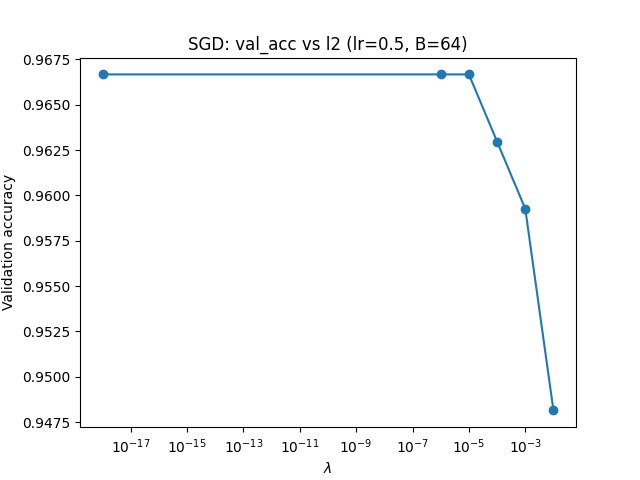
\includegraphics[scale=0.5]{plots/valacc-vs-l2.png}
    \caption{Final validation accuracy vs. $L^2$ regularization parameter for SGD}
\end{figure}

\subsubsection{Learning rate}\;\\
We also studied the effect of the learning rate on convergence speed by comparing validation accuracy as a function of wall-clock time for both SGD and full-batch GD. In these runs, we fixed the regularization strength to $\lambda=0$ and, for SGD, we fixed the batch size to $B=64$.

\begin{figure}[H]
    \centering
    \begin{tabular}{cc}
        
\includegraphics[width=0.49\textwidth]{plots/valacc-vs-time-vs-lr-SGD.png} &
        
\includegraphics[width=0.49\textwidth]{plots/valacc-vs-time-vs-lr-FGD.png}
    \end{tabular}
    \caption{Validation accuracy vs.\ time for different learning rates in SGD (left) and full-batch GD (right).}
    \label{fig:learning_rate_tuning}
\end{figure}

As expected, the learning rate strongly affects the convergence behavior of both methods: smaller values yield slower progress, while larger values reach high accuracy in fewer seconds (up to the stability limit) \cite[Ch. 11.4.1]{Goodfellow2016}. In this setup, SGD reaches a high validation accuracy substantially faster than full-batch GD, while achieving comparable final performance.

\subsubsection{Batch size}\;\\
We next investigated the effect of the mini-batch size $B$ on the validation accuracy of SGD, keeping $\lambda=0$ and $\alpha=0.5$ fixed (Figure~\ref{fig:batch_size_tuning}). The batch size influences both the stochasticity of the gradient estimate and the number of parameter updates performed per epoch (approximately $n/B$), so the comparison reflects both optimization dynamics and the imposed training budget.

In our runs, intermediate batch sizes performed best: accuracy improves from very small batches up to $B\approx 64$--$128$, while larger batches show a slight degradation. This is consistent with the usual trade-off between noisy but frequent updates for small $B$ and smoother but less frequent updates for large $B$, under a fixed epoch budget. \cite[Ch. 8.1.3]{Goodfellow2016}

\begin{figure}[H]
    \centering
    
\includegraphics[scale=0.5]{plots/valacc-vs-batchsize.png}
    \caption{Validation accuracy vs.\ batch size for SGD ($\lambda=0$, $\alpha=0.5$).}
    \label{fig:batch_size_tuning}
\end{figure}

For this sweep we used a fixed maximum number of epochs and enabled threshold stopping when the validation accuracy reached $0.96$ (with the configured patience). The best configuration in this grid is $B=64$ (Figure~\ref{fig:batch_size_tuning}).


\subsection{Final models and discussion}\;\\
We finally compare the two selected configurations (SGD and full-batch GD) after training on the combined train+validation set, and report performance on the held-out test set. The confusion matrices in Figure~\ref{fig:confusion_matrices} show that both methods achieve strong test performance, with most mass concentrated on the diagonal and only a small number of misclassifications.

\begin{figure}[H]
    \centering
    \begin{tabular}{cc}
        
\includegraphics[width=0.49\textwidth]{plots/confusion-sgd.png} &
        
\includegraphics[width=0.49\textwidth]{plots/confusion-fgd.png}
    \end{tabular}
    \caption{Confusion matrices on the test set for the final SGD model (left) and the final full-batch GD model (right).}
    \label{fig:confusion_matrices}
\end{figure}

To compare optimization behavior, Figure~\ref{fig:objective_and_gap} reports the objective value and the corresponding optimality gap as a function of effective data passes. In this experiment, SGD reduces the objective more rapidly during the initial phase, which is consistent with its frequent parameter updates based on mini-batches. Full-batch GD follows a smoother trajectory because it uses the exact full gradient at every step, but each iteration is computationally heavier.

\begin{figure}[H]
    \centering
    \begin{tabular}{cc}
        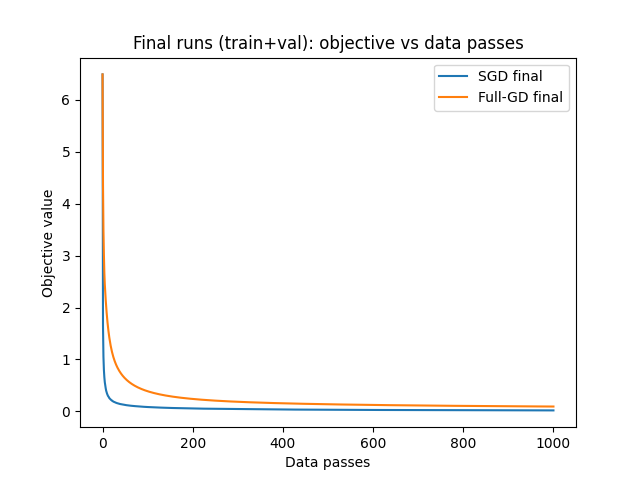
\includegraphics[width=0.49\textwidth]{plots/final-run-obejctiv-vs-data-passes.png} &
        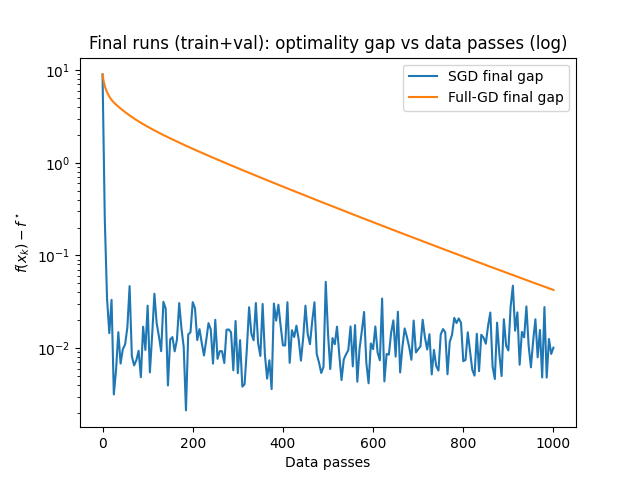
\includegraphics[width=0.49\textwidth]{plots/final-run-optimalitygap-vs-data-passes.png}
    \end{tabular}
    \caption{Objective value (left) and optimality gap (right, log scale) vs.\ data passes for the final SGD and full-batch GD runs (trained on train+val).}
    \label{fig:objective_and_gap}
\end{figure}

In the optimality-gap plot, the reference value $f^\star$ is computed empirically as the minimum objective observed along a long fixed-step full-batch GD run. This value should therefore be interpreted as a numerical baseline rather than a certified optimum. In our experiments, the final SGD run achieves a lower training objective than this reference, i.e.\ $f_{\mathrm{SGD}} < f^\star$, indicating that the chosen reference run does not attain the best objective value encountered in our study. Consequently, the plotted ``gap'' mainly reflects proximity to this baseline and is sensitive to how the reference $f^\star$ is constructed.

Overall, for problems where full gradients are expensive (large $n$ and/or high-dimensional models), SGD (or mini-batch variants) is typically preferred due to its lower per-update cost and favorable time-to-accuracy. Full-batch GD can be attractive when the dataset is small enough that full gradients are cheap, since its updates are deterministic and its objective trajectory is smoother.